\documentclass[aspectratio=1610]{beamer}
\usepackage{graphicx}
\usepackage{amsmath}
\usepackage{amsfonts}
\usepackage{tikz}

% BibLaTeX setup
\usepackage[backend=biber,style=authoryear-comp,sorting=nyt]{biblatex}
\addbibresource{refere.bib}

\usecolortheme{default}

\title{Validation of Coupled Atmospheric-Aeroelastic Model System for Wind Turbine Power and Load Calculations}
\subtitle{Application to Enercon Wind Turbines}
\author{Aravind Venkatachalapathy}
\institute{Enercon}
\date{\today}

\begin{document}

% Slide 1: Title Slide
\frame{\titlepage}

% Slide 2: Introduction and Motivation
\begin{frame}{Introduction and Motivation}
    \begin{columns}
        \begin{column}{0.6\textwidth}
            \textbf{Research Objective:}
            \begin{itemize}
                \item Validate coupled atmospheric- aeroelastic models for accurate wind turbine simulations.
                \item Focus on Enercon turbine technology and performance
            \end{itemize}
            \textbf{Traditional Aeroelastic Simulation Limitations:}\\
             \textcolor{red}{Synthetic turbulence (Kaimal/Mann spectrum) models} :
                \begin{itemize}
                    \item Assume statistically stationary, homogeneous turbulence
                    \item Pre-calculated wind fields with simplified atmospheric conditions
                    \item Limited representation of complex flow phenomena (gusts, shear, atmospheric stability)
                \end{itemize}
        \end{column}
        \begin{column}{0.4\textwidth}
                \textcolor{red}{Wake modeling deficiencies:}
                \begin{itemize}
                    \item Simplified wake models (Jensen, Frandsen) lack temporal dynamics
                    \item No feedback between turbine operation and atmospheric flow
                \end{itemize}
            
            \vfill
            \begin{center}
              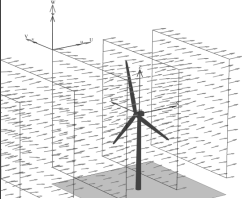
\includegraphics[width=0.7\textwidth]{wind.png}  
            \end{center}
            
            
        \end{column}
    \end{columns}
\end{frame}

% Slide: Actuator Sector Model (ASM) - Concept and Motivation
\begin{frame}{Actuator Sector Model (ASM) - Concept and Motivation}
    \begin{columns}
        \begin{column}{0.6\textwidth}
                \textcolor{red}{ALM Limitations:}
                \begin{itemize}
                \small
                    \item Small time steps required ($\Delta t_F$)
                    \item High computational cost for LES
                \end{itemize}
                
                \textcolor{blue}{ADM Advantages:}
                \begin{itemize}
                \small
                    \item Larger time steps possible
                    \item Lower computational cost
                    \item No individual blade information
                \end{itemize}
                
                \textcolor{green}{ASM Solution:}
                \begin{itemize}
                \small
                    \item Detailed blade output + Computational efficiency
                    \item Decoupled time stepping
                \end{itemize}

            
            \textbf{Time Step Decoupling Strategy:}
            \begin{itemize}
            \small
                \item PALM: $\Delta t_P$ determined by CFL/diffusion criteria
                \item FAST: $\Delta t_F < \Delta t_P$ for ALM accuracy
                \item Significant reduction in total computational time
            \end{itemize}
        \end{column}
        
        \begin{column}{0.4\textwidth}
        \begin{center}
          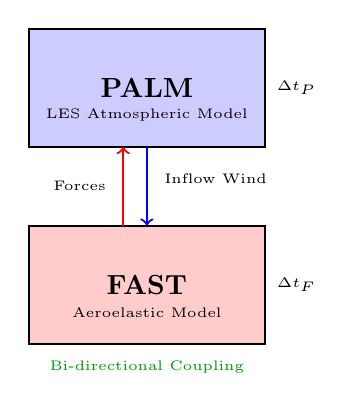
\begin{tikzpicture}
    % PALM box
    \draw[fill=blue!20, thick] (0,3) rectangle (3,4.5);
    \node at (1.5,3.75) {\textbf{PALM}};
    \node[font=\tiny] at (1.5,3.4) {LES Atmospheric Model};
    
    % FAST box
    \draw[fill=red!20, thick] (0,0.5) rectangle (3,2);
    \node at (1.5,1.25) {\textbf{FAST}};
    \node[font=\tiny] at (1.5,0.9) {Aeroelastic Model};
    
    % Arrow from PALM to FAST (Inflow wind)
    \draw[->, thick, blue] (1.5,3) -- (1.5,2);
    \node[font=\tiny, right] at (1.6,2.6) {Inflow Wind};
    
    % Arrow from FAST to PALM (Forces)
    \draw[->, thick, red] (1.2,2) -- (1.2,3);
    \node[font=\tiny, left] at (1.1,2.5) {Forces};
    
    % Time step indicators
    \node[font=\tiny] at (3.4,3.75) {$\Delta t_P$};
    \node[font=\tiny] at (3.4,1.25) {$\Delta t_F$};
    
    % Coupling indication
    \node[font=\tiny, green!60!black] at (1.5,0.2) {Bi-directional Coupling};
\end{tikzpicture}  
        \end{center}

            
            \vspace{0.3cm}
            \small
            ASM allows PALM to use optimal atmospheric time steps while maintaining detailed turbine physics in FAST
        \end{column}
    \end{columns}
\end{frame}

% Slide: ASM Implementation and Technical Details
\begin{frame}{ASM Operational Mechanism}
    \begin{columns}
        \begin{column}{0.6\textwidth}
            \textbf{ASM Operational Steps:}
            \begin{enumerate}
                \item FAST communicates initial blade positions
                \item PALM provides wind speeds from frozen field
                \item During $\Delta t_P$, rotor sweeps sector: 
                $$\phi = \Omega \cdot \Delta t_P$$
                \item Forces from central blade line applied to entire sector
                \item Multiple FAST calculations per PALM time step
            \end{enumerate}
            
            \vspace{0.3cm}
            \begin{block}{Technical Benefits}
                \begin{itemize}
                    \item Maintains ALM physics in FAST
                    \item Efficient force projection in PALM
                \end{itemize}
            \end{block}
            %\textbf{Force Distribution (Gaussian Smearing):}
            %$$\eta = \frac{1}{\epsilon^3 \pi^{3/2}} \exp\left(-\frac{r^2}{\epsilon^2}\right)$$
            %where $\epsilon = 2\Delta$ (grid spacing factor)
        \end{column}
        
        \begin{column}{0.4\textwidth}
            \begin{figure}
                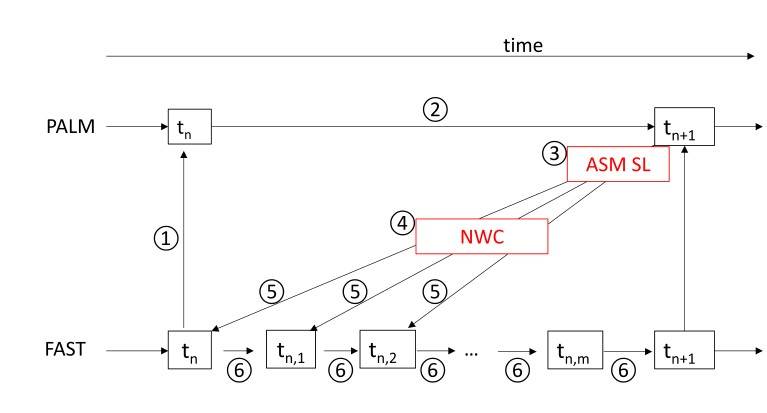
\includegraphics[width=\textwidth]{ASM.jpg}
                \caption{Schematic of the operation mode of the coupling}
                \label{fig:asm_sector}
            \end{figure}
            Based on research work done by \cite{steinbruck2024}, \cite{kruger2022}
        \end{column}
    \end{columns}
\end{frame}

\begin{frame}{Intended Outcomes}

\end{frame}
\begin{frame}{References}
    \printbibliography
\end{frame}
\end{document}
